\graphicspath{{figs/3c}}

\chapter{Uncertainty Applications}
In this chapter, we address a significant concern in neural networks: their tendency to exhibit overconfidence in predictions. We tackle this issue by exploring uncertainty estimation techniques, notably highlighting the capabilities of Monte-Carlo Dropout variational inference, which was introduced in the previous chapter. These methods play a crucial role in mitigating overconfidence, particularly in scenarios where accurate uncertainty estimation is essential, such as failure prediction and the identification of out-of-distribution instances. This concluding chapter aims to offer a deeper comprehension and practical experience in understanding how Bayesian methods can assist us in effectively managing neural network overconfidence.

\section{Monte-Carlo Dropout on MNIST}
In this section, we focus on training a model using Monte Carlo Dropout (MC Dropout) on the MNIST dataset and analysing the behaviour of the outputed probabilities for certain and uncertain samples. To find out the most uncertain images, we used the variation ratio metric, which effectively measures epistemic uncertainty and is straightforward to calculate. For a given image, denoted as $ \mathbf{x} $, we perform $ T $ stochastic forward passes through the model and record the predicted labels. We then determine the frequency $ f^{c^\star }_\mathbf{x} $ of the most common label ($ c^\star $) across the $ T $ passes. The variation ratio for image $ \mathbf{x} $ is calculated using the formula:
\[
    \text{var-ratio}[\mathbf{x}] = 1 - \frac{f^{c^\star }_\mathbf{x}}{T}
.\]
This formula provides a quantitative measure of uncertainty for an image.

\paragraph*{1.1. What can you say about the images themselfs? How do the histograms along them helps to explain failure cases? Finally, how do probabilities distribution of random images compare to the previous top uncertain images?}
In this experiment, we utilized a LeNet-5 style model with Monte-Carlo dropout for variational inference, training it on the MNIST dataset for 20 epochs using standard cross-entropy. We then applied the model to calculate variation ratios for each test image, enabling us to sort images based on their uncertainty. These images are displayed in \Cref{fig:varratio_certain,fig:varratio_certain}, accompanied by five types of measurements derived from the model's probability outputs. To summarize how the output probabilities fluctuate across $ T=100 $ stochastic forward passes, we used histograms depicting three different distributions:
\begin{enumerate}
    \item The first column shows the distribution of the mean output probability for each class.
    \item The second column displays the distribution of the predicted class across the $ T $ forward passes.
    \item The last three columns present the distribution of the output probability for specific classes (the most predicted class for the third column, the ground truth class for the fourth, and a different class for the fifth).
\end{enumerate}
These histograms illustrate the variability of output probabilities across the $ T=100 $ iterations. A model lacking confidence in its prediction will show this through greater variation in output probabilities between draws, resulting in more dispersed histograms and changes in the predicted class. Conversely, a confident model will have much more concentrated histograms, with the predicted class remaining the same across all iterations.

\Cref{fig:varratio_certain} displays images deemed certain by the model. To the human eye, these images clearly belong to their assigned classes. The distributions here are characterized by a single peak, indicating the same value is drawn repeatedly. The mean probabilities for the predicted class equal one, and all other classes consistently have a zero probability, suggesting the model is very confident in its predictions.

Conversely, \Cref{fig:varratio_uncertain} shows images classified as uncertain by the model. These images appear more ambiguous, and even to the human eye, it can be challenging to determine their actual numbers. The distributions here are more spread out. This implies various output class neurons may be activated, either simultaneously or independently at various levels in each run. To gain a deeper understanding of this phenomenon, we examine the distribution of the predicted class along with the mean probabilities. The similarity between these two histograms suggests that the model may select a certain class as the prediction even when the average probability for that class is relatively low. We explored two possible explanations for this:
\begin{itemize}
    \item The mean don't tell the full story. A small mean for a class doesn't necessarily imply the class neuron never reaches high values. Indeed, the last column shows that "small mean" classes (eg. class 8) can occasionally reach values around $0.8$, increasing their likelihood of being predicted. This can also easily be observed on \Cref{fig:proba_barplot}, where a lot of high value outliers are present. 
    \item The class neuron may sometimes record low values, but it is still the highest compared to other class neurons.
\end{itemize}
To verify these hypotheses, we plotted the Maximum Class Probability (MCP) in \Cref{fig:MCP}. MCP, which is the probability used for making the prediction, is defined as $ \text{MCP}(\boldsymbol{x}) = \max _{k \in \mathcal{Y}} p(Y=k | \boldsymbol{w}, \boldsymbol{x}) $ and serves as a basic confidence baseline. \Cref{fig:MCP:barplot} reveals that most predictions for the image were based on high probability, even though it's often misclassified and considered one of the most uncertain images in the dataset. This highlights the model's overconfidence. However, sometimes a decision is made at a lower probability, such as below $ 0.4 $. The subsequent plot in \Cref{fig:MCP:kdeplot} helps identify which class the model tends to predict when the MCP is either low or high. For instance, class 8 is consistently predicted with a high MCP, whereas class 7 is always associated with a low MCP.

\begin{figure}[H]
    \centering
    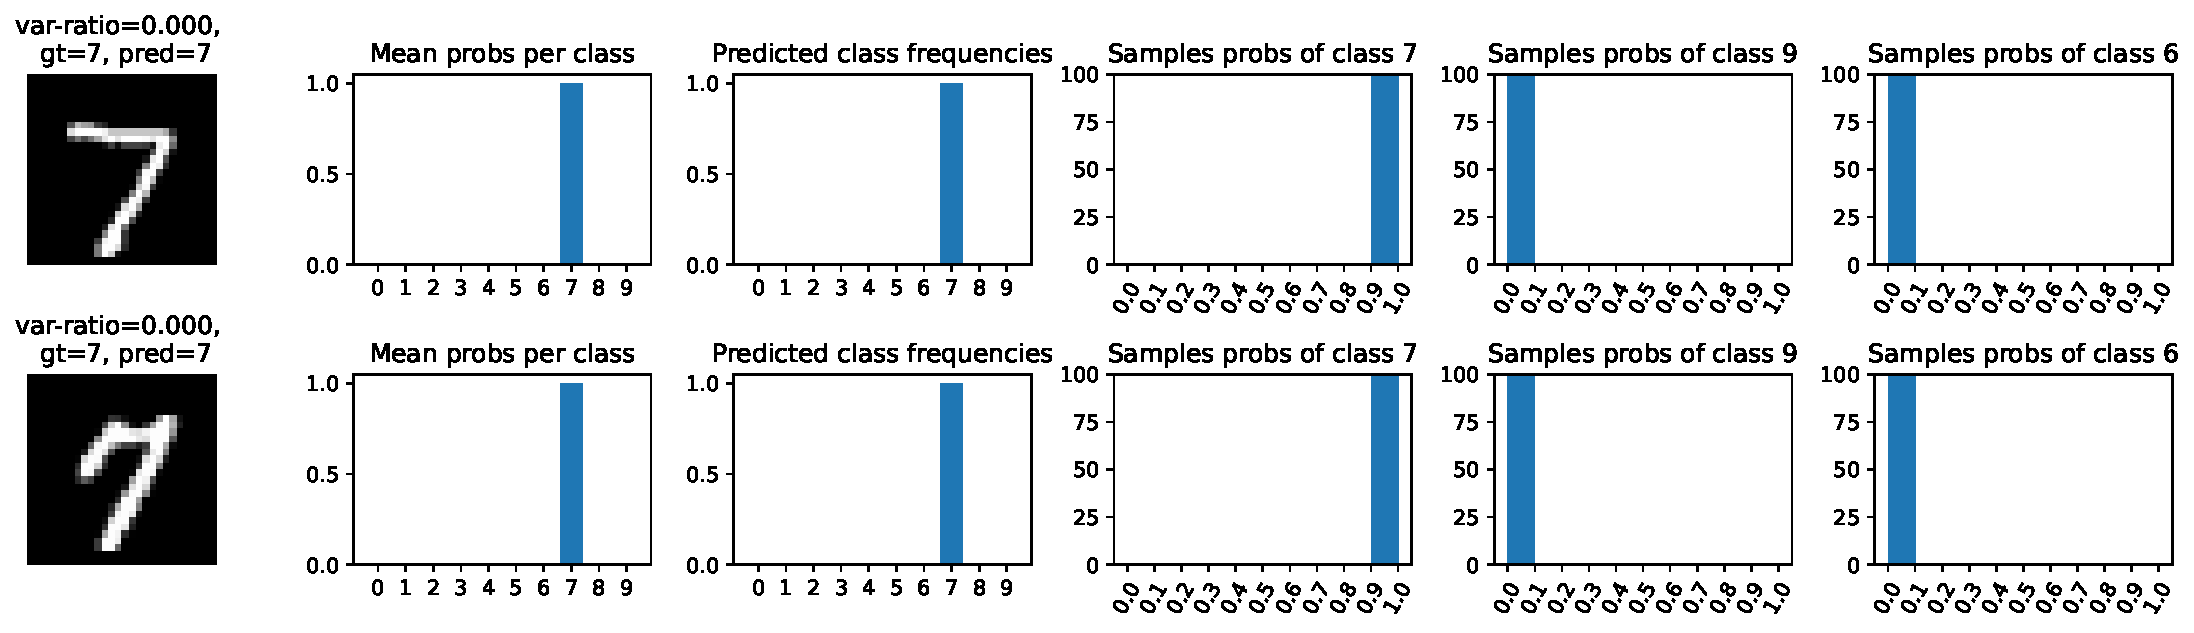
\includegraphics[width=0.95\textwidth]{var-ratio_certain_images.pdf}
    \caption{\textbf{Certain images with output probability distributions.} Images that the model classified with high certainty, featuring clear, identifiable digits. Histograms show highly concentrated distributions, with mean probabilities for the predicted class at one and other classes at zero, indicating strong model confidence in its predictions.}
    \label{fig:varratio_certain}
\end{figure}
\begin{figure}[H]
    \centering
    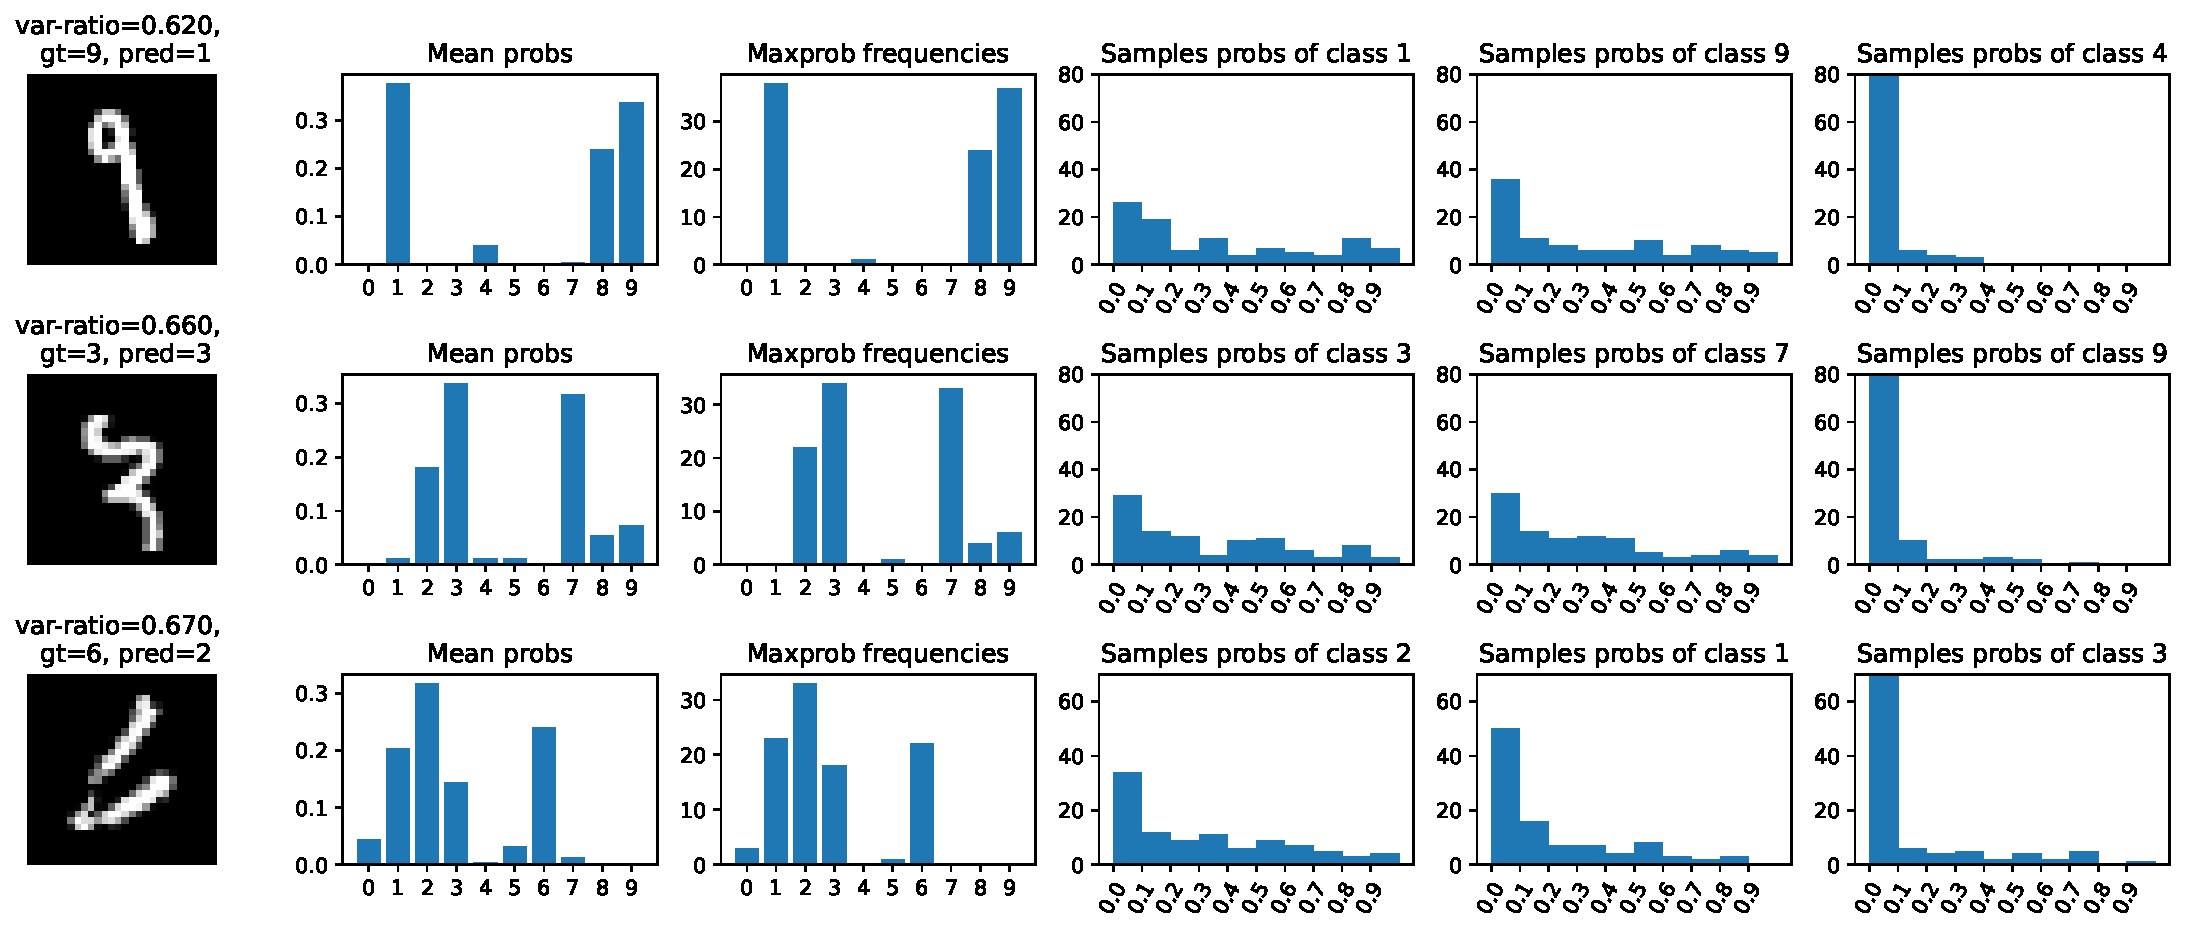
\includegraphics[width=0.95\textwidth]{var-ratio_uncertain_images.pdf}
    \caption{\textbf{Uncertain images with output probability distributions.} Ambiguous images that the model classified with uncertainty. Distributions are spread out, suggesting fluctuating confidence across different classes. The similarity between histograms of the predicted class and mean probabilities indicates that the model sometimes chooses a class with a relatively low average probability.}
    \label{fig:varratio_uncertain}
\end{figure}
\begin{figure}[H]
    \centering
    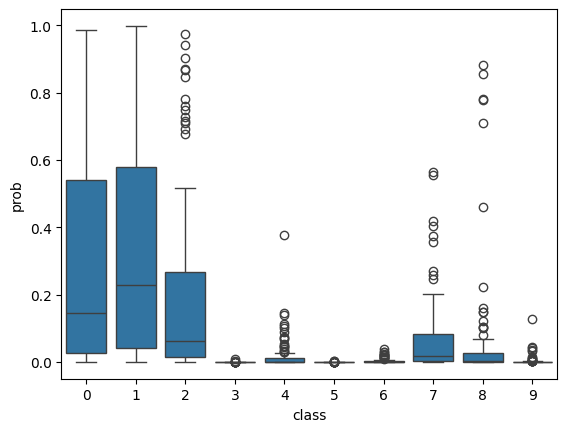
\includegraphics[width=0.45\textwidth]{proba_barplot.png}
    \caption{\textbf{Box plot visualization of the probability distribution of each class for $ T=100 $ draw.}}
    \label{fig:proba_barplot}
\end{figure}

\begin{figure}[H]
    \centering
    \begin{subfigure}{0.45\textwidth}
        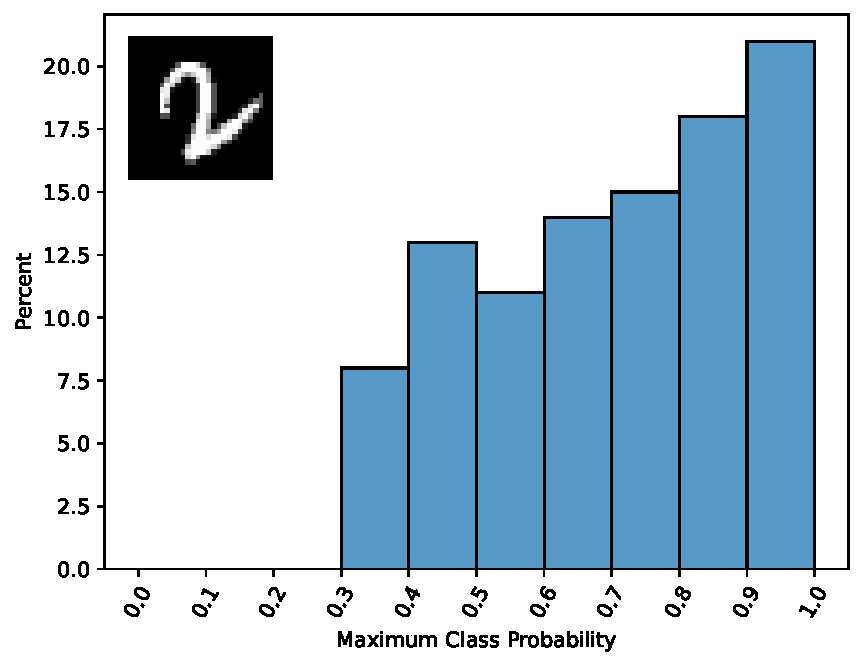
\includegraphics[width=\textwidth]{MCP_barplot.pdf}
        \caption{}
        \label{fig:MCP:barplot}
    \end{subfigure}%
    \begin{subfigure}{0.45\textwidth}
        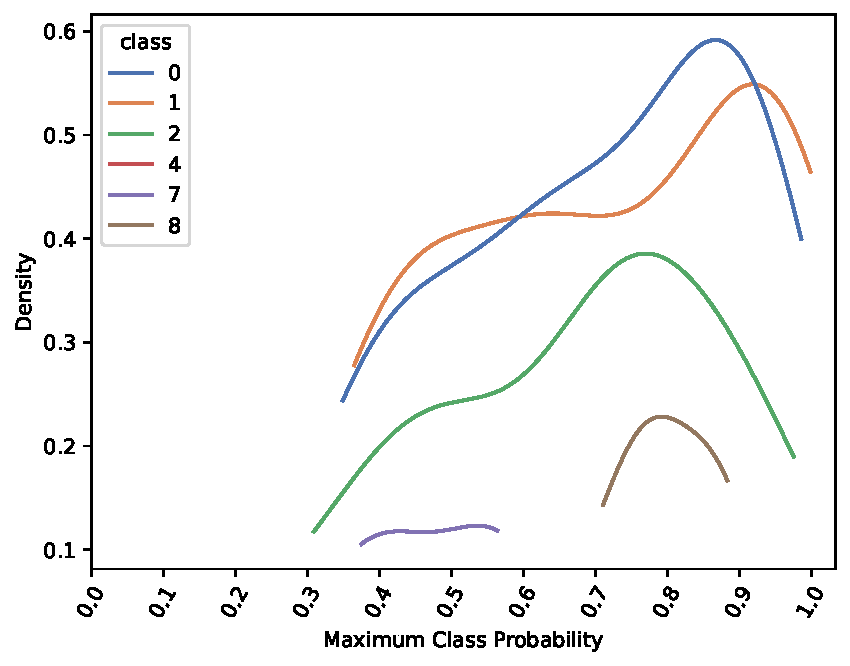
\includegraphics[width=\textwidth]{MCP_kdeplot.pdf}
        \caption{}
        \label{fig:MCP:kdeplot}
    \end{subfigure}%
    \caption{\textbf{(a) Bar plot of Maximum Class Probability.} Bar plot showcasing the Maximum Class Probability (MCP) for uncertain images. It reveals that most predictions are based on high probability, pointing to model overconfidence. However, some decisions are made at lower probabilities, suggesting inconsistency in the model's confidence level.\\\textbf{(b) Density plot of Maximum Class Probability in function of the class.} KDE plot illustrating the distribution of MCP for different preditected classes, indicating the model's tendency to predict certain classes with high MCP (e.g., class 8) and others with consistently low MCP (e.g., class 7), reflecting the model's varying confidence across different classes.}
    \label{fig:MCP}
\end{figure}

\section{Failure prediction}
In this section, we have conducted a comparison of various methods aimed at obtaining a reliable confidence measure for model predictions. Such a measure permit to distinguish correct and incorrect prediction and so identify instances where a machine learning model does not perform as expected or fails to make accurate predictions. Failure in a machine learning context can occur due to various reasons, such as poor model training, noisy or out of distribution data, inadequate feature representation, overfitting or underfitting. An intelligent decision system equipped with such metrics in operational settings can make informed choices, including adhering to the model's prediction or, conversely, involving a human operator, activating a backup system equipped with additional sensors, or triggering an alarm. This field of application is commonly referred to as failure prediction.

During the lecture and in the previous section, we found that Maximum Class Probability (MCP) is not a great metric for failure prediction. It assigns high confidence values to both correct and erroneous predictions because modern models tend to be overconfident, resulting in overlapping distributions between successes and errors. This issue persists even when using temperature scaling calibration.

Alternatively, when the model makes a misclassification, the probability associated with the true class $y$ tends to be lower than the maximum probability, often falling to a low value. This observation leads us to consider the True Class Probability (TCP) as a suitable measure of uncertainty. However, the true class labels $y$ are not available when estimating confidence for test inputs. This motivates the development of ConfidNet, whose primary objective is to directly regress the TCP value from the input image, allowing us to obtain a reliable measure of uncertainty without access to ground truth labels.

In this practical section, we implemented ConfidNet to address failure predictions and compared it to two other methods that rely solely on the model's output probabilities. The first method is MCP, and the second is the entropy of the output probabilities. For these two methods, we used the previously trained MC Dropout model to compute the output probabilities. ConfidNet was trained for 30 epochs with the previous MC Dropout model as a teacher with frozen parameters and Mean Squared Error as the loss function.

\paragraph*{2.1. Compare the precision-recall curves of each method along with their AUPR values. Why did we use AUPR metric instead of standard AUROC?}
To assess and compare these methods, we require a suitable metric. Our objective is to identify classification errors, which we consider as the positive detection class, while correct predictions serve as the negative detection class. Since our models excel at making accurate predictions, we anticipate a low occurrence of classification errors, resulting in an imbalanced setting with a significant number of true negatives.

We have opted to employ the AUPR (Area Under the Precision-Recall Curve) instead of the AUROC (Area Under the Receiver Operating Characteristic Curve) due to the latter's unsuitability for imbalanced datasets. AUROC treats both classes equally and can yield misleading results, particularly under the influence of a large number of true negatives. This may overstate the model's performance, particularly in distinguishing the minority class, which in this context comprises classification errors. Conversely, AUPR is a more suitable choice, as it prioritizes precision and recall for the minority class. Precision measures the fraction of actual positives among the positive predictions, while recall measures the proportion of correctly identified actual positives. Consequently, AUPR proves to be a more reliable metric in our situation, where the positive class (classification errors) is significantly smaller than the negative class (correct predictions).

\Cref{fig:failure_aupr} illustrates the precision-recall curves for each method, accompanied by their respective AUPR values. The results demonstrate that ConfidNet surpasses the other two methods. This superiority can be attributed to ConfidNet's training, which directly estimates the TCP value—a more dependable uncertainty measure compared to MCP and entropy, as elaborated upon in the section introduction. Notably, ConfidNet exhibits a slower decline in precision as recall increases, indicating a more balanced performance in terms of identifying true positives without a substantial rise in false positives.

For a better understanding of the lecture's confidence metrics, we aimed to compare the performance of predictive entropy and mutual information in the context of failure detection. The results are presented in \Cref{fig:failure_aupr_entropy_vs_mut_inf}. It seems that entropy outperforms mutual information as a metric for failure detection. This distinction arises from the fact that predictive entropy measures aleatoric uncertainty, while mutual information assesses epistemic uncertainty. In the specific experiment of failure detection on MNIST, it proves more advantageous to rely on and measure aleatoric uncertainty, which originates from the natural variability or randomness of the numbers in the images. This explanation underscores why entropy is a superior metric to mutual information in this particular context.
\begin{figure}[H]
    \centering
    \begin{subfigure}{0.45\textwidth}
        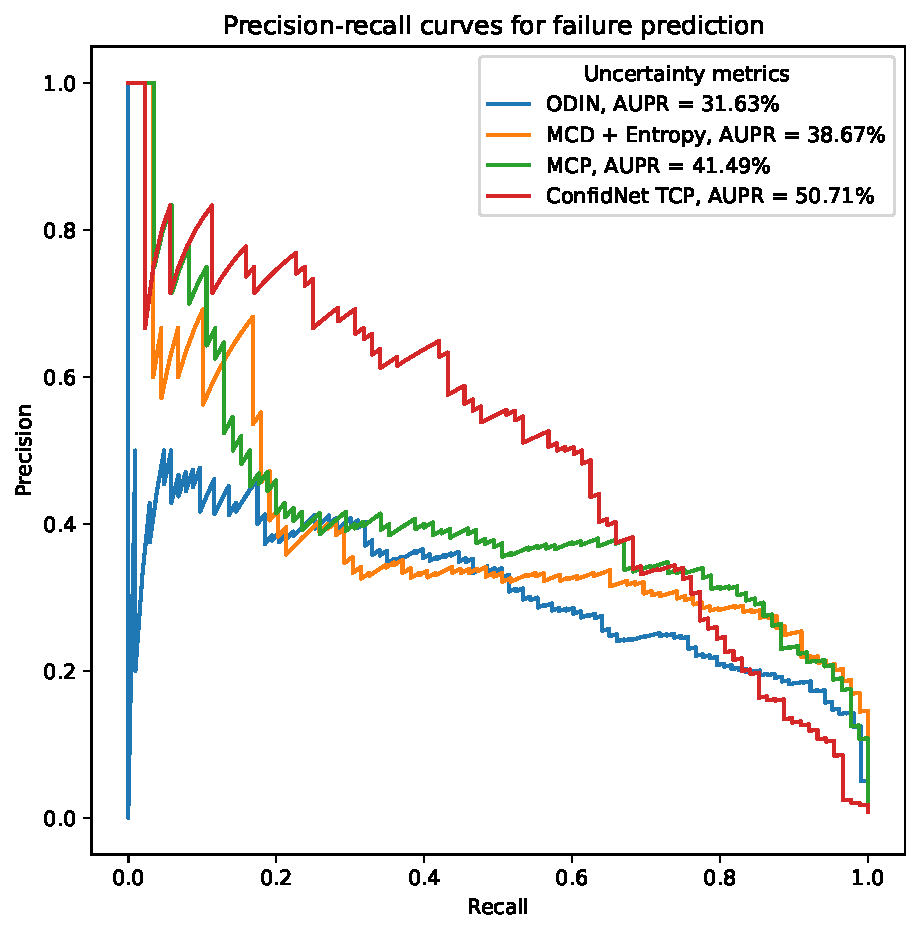
\includegraphics[width=\textwidth]{failure_aupr.pdf}
        \caption{}
        \label{fig:failure_aupr}
    \end{subfigure}%
    \begin{subfigure}{0.45\textwidth}
        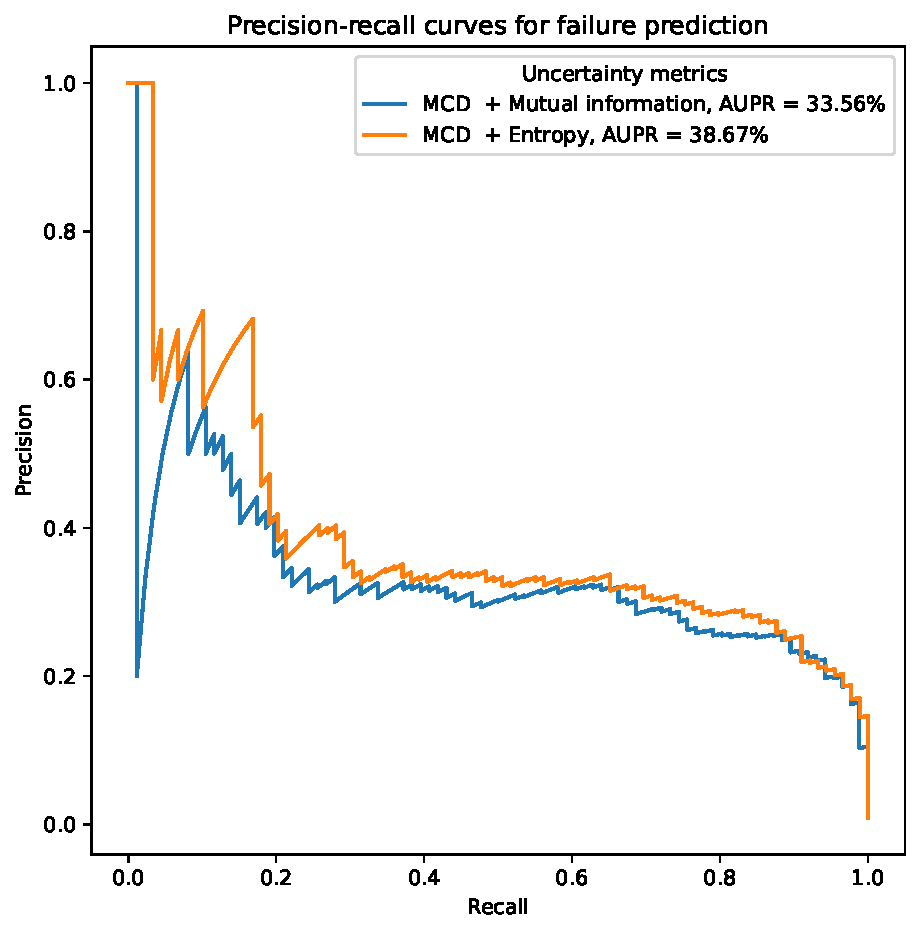
\includegraphics[width=\textwidth]{failure_aupr_entropy_vs_mut_inf.pdf}
        \caption{}
        \label{fig:failure_aupr_entropy_vs_mut_inf}
    \end{subfigure}%
    \caption{\textbf{(a) Precision-recall curves for each tested method with AUPR values.} The graph demonstrates ConfidNet's balanced performance in identifying true positives with fewer false positives, indicating its effectiveness in making accurate predictions with a low occurrence of classification errors.\\\textbf{(b) Performance comparison of predictive entropy and mutual information for failure detection.} The graph illustrates that predictive entropy, measuring aleatoric uncertainty, outperforms mutual information, which measures epistemic uncertainty. This suggests that in scenarios with aleatoric uncertainty, like natural variability in MNIST images, entropy is a more effective metric for failure detection.}
\end{figure}

\section{Out-of-distribution detection}
In today's machine learning landscape, models are often trained on vast datasets, such as ImageNet, which can reduce epistemic uncertainty. However, in critical real-world applications like autonomous driving, the need to identify out-of-distribution (OOD) inputs remains essential due to the infinite variability of real-life data. OOD detection plays a crucial role because machine learning models typically assume that the data they encounter during real-world predictions will resemble the data they were trained on. When a model confronts data that significantly deviates from its training data, it can result in unpredictable and unreliable predictions. OOD detection aims to identify such situations, allowing for cautious handling or even disregarding of the model's predictions on such atypical data. It's important to note that while OOD data can lead to model failure, not all model failures are solely attributed to OOD data. Model failures can occur for various reasons, including overfitting, underfitting, or architectural issues, even when the data falls within the expected distribution. Therefore, while OOD detection is a critical component of ensuring a model's robustness, it represents just one facet of the broader spectrum of failure detection within machine learning systems.

In this section, we will find out what's the best methods for OOD detection. We will use the Kuzushiji-MNIST (KMNIST) dataset as out-of-distribution data for our MC dropout MNIST predictor. This dataset consists of 70,000 28x28 grayscale handwritten Hiragana images. We will evaluate the performance using precision, recall, and AUPR as metrics to compare different methods.

Specifically, in this section, we have implemented the ODIN method \citep{ODIN}, which enhances maximum softmax probabilities with temperature scaling and inverse adversarial perturbation. These techniques are employed to increase the distinction between in-distribution and out-of-distribution data.\\
Temperature scaling involves applying a simple scaling of the logit by a temperature parameter $ \nicefrac{1}{T} $ before the softmax: $ S_i(\boldsymbol{x}, T) = \frac{\exp (f_i(\boldsymbol{x}) / T)}{\sum_{j=1}^{N} \exp (f_j(\boldsymbol{x} / T))} $, where $ S_i $ represents the output probabilities, $ \boldsymbol{x} $ is the input image, $ T $ is the temperature parameter, and $ f_i $ is the logit of the $ i $-th class.\\
Inverse adversarial perturbation is used to preprocess the input $ \boldsymbol{x} $ before feeding it to the neural network. This preprocessing involves adding a small perturbation to the input image $ \boldsymbol{x} $ such that $ \boldsymbol{x}^\prime = \boldsymbol{x} - \epsilon \cdot \text{sign}(-\nabla_{\boldsymbol{x}} \mathcal{L}(\boldsymbol{x}, y)) $, where $ \mathcal{L} $ is the cross-entropy loss function, $ y $ is the ground truth label, $ \epsilon $ is the perturbation magnitude, and $ \boldsymbol{x}^\prime $ is the perturbed image. The perturbation magnitude $ \epsilon $ is chosen to ensure the perturbed image remains correctly classified by the neural network.

\paragraph*{3.1. Compare the precision-recall curves of each OOD method along with their AUPR values. Which method perform best and why?}
\Cref{fig:OOD_aupr} displays the precision-recall curves for six uncertainty metrics (MCP, ODIN, CondifNet TCP, MC Dropout (MCD) mutual information, and MCD predictive entropy), along with their corresponding AUPR values. Given the smoothness of these curves, our analysis will primarily focus on the AUPR values.

ODIN, with its two modifications to output probabilities, performs slightly better than MCP, which aligns with expectations since ODIN builds upon MCP. However, ODIN is surprisingly surpassed by the other two MCD methods. This outcome was not anticipated for mutual information and predictive entropy since they, like ODIN, depend on the raw output probabilities. These methods appear to benefit from the stochastic nature of MC Dropout. In fact, both methods achieved impressive AUPR scores of $98\%$, ranking as the most effective metrics for OOD detection. In our previous experiment, although ConfidNet emerged as the top method for detecting failures, it showed a marginal lag, achieving an AUPR of $96\%$. This can be readily understood when considering that there is no TCP available for out-of-distribution data. Consequently, ConfidNet lacks specific data to predict or train on in these scenarios. Mutual information and predictive entropy, despite their simplicity, emerge as leading metrics for OOD detection in our experiments, but at the expense of a more complex (Bayesian) network. For instance, computing the entropy score takes 18 seconds, whereas ODIN requires only 4.1 seconds.
\begin{figure}[H]
    \centering
    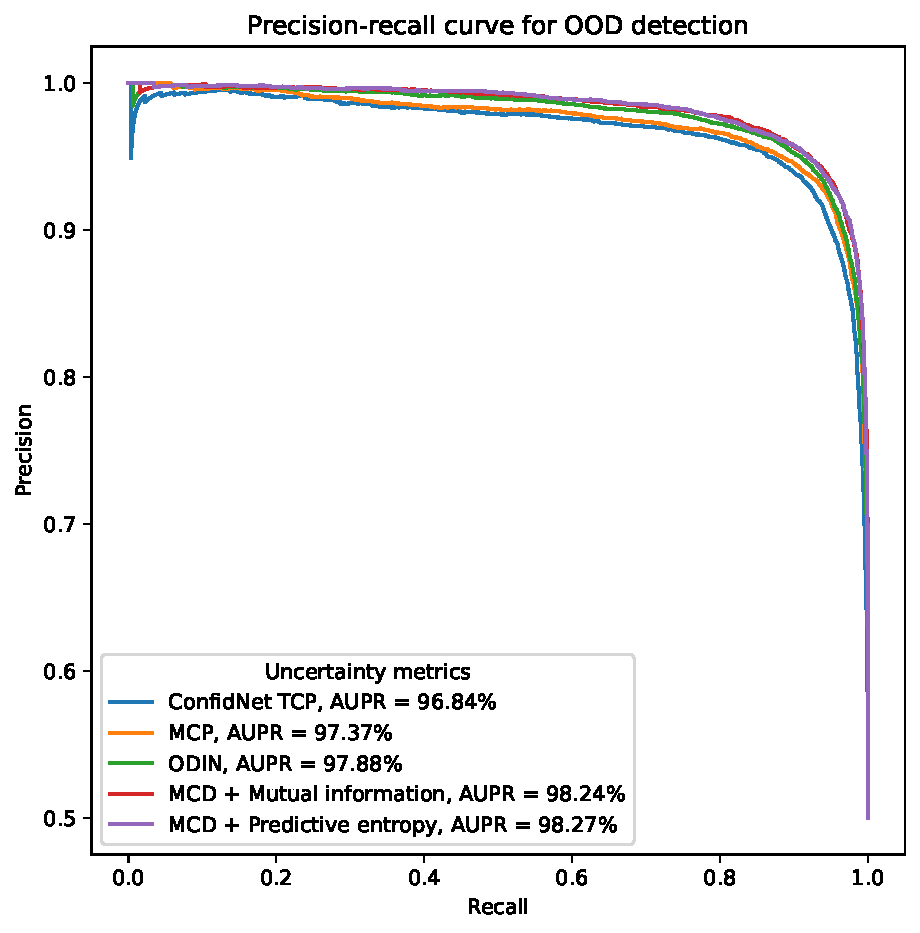
\includegraphics[width=0.45\textwidth]{OOD_aupr.pdf}
    \caption{\textbf{Precision-recall curves and AUPR values for six uncertainty metrics.} Precision-recall curves for six uncertainty metrics (MCP, ODIN, ConfidNet TCP, MC Dropout (MCD) mutual information, and MCD predictive entropy) with their corresponding Area Under the Precision-Recall curve (AUPR) values. MCD mutual information and predictive entropy lead with AUPR scores of $98\%$. ODIN performs slightly better than MCP but is outperformed by MCD methods, which take advantage of Bayesian networks. However, note that the performance of MCD methods comes at a computational cost.}
    \label{fig:OOD_aupr}
\end{figure}

To further investigate ODIN's techniques, we attempted to combine them with MC Dropout (averaging over 100 stochastic forward passes), predictive entropy, and mutual information. The outcomes are presented in \Cref{fig:OOD_aupr_combo}. This combination actually resulted in a slight performance decline for Entropy and Mutual Information, with a decrease of approximatly $0.3\%$ in their scores. Integrating MCD with ODIN appears to have no significant impact.
\begin{figure}[H]
    \centering
    \begin{subfigure}{0.45\textwidth}
        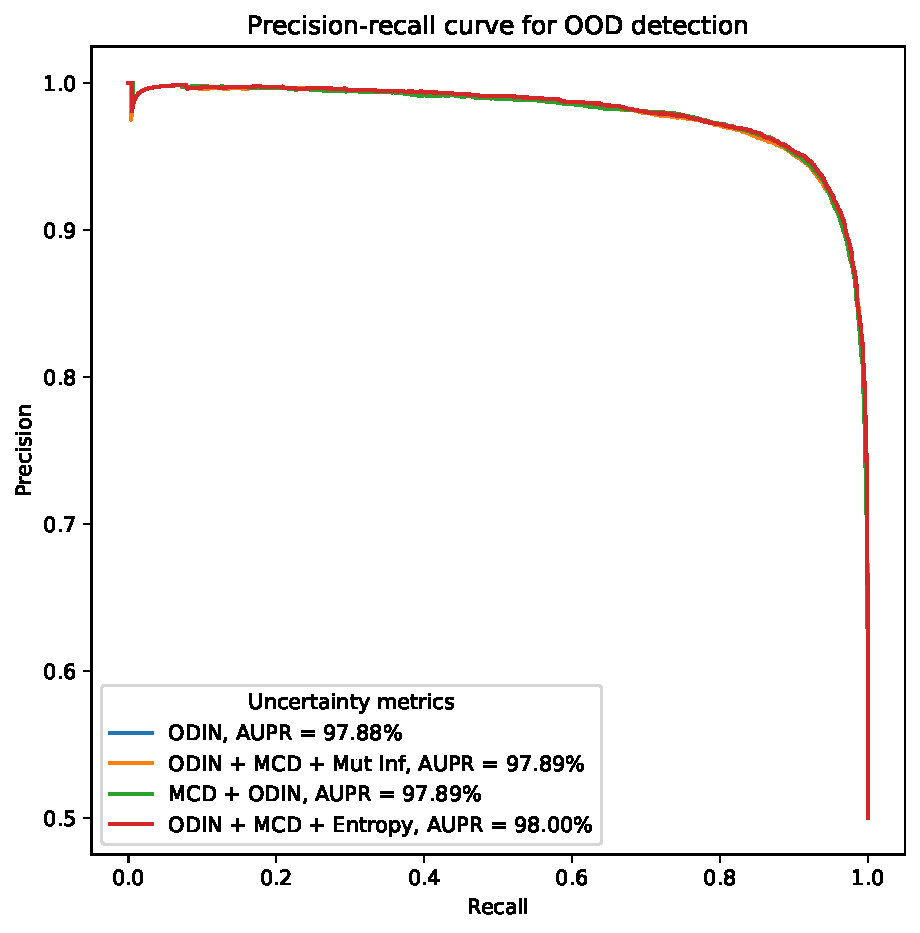
\includegraphics[width=\textwidth]{OOD_aupr_combo.pdf}
        \caption{}
        \label{fig:OOD_aupr_combo}
    \end{subfigure}%
    \begin{subfigure}{0.45\textwidth}
        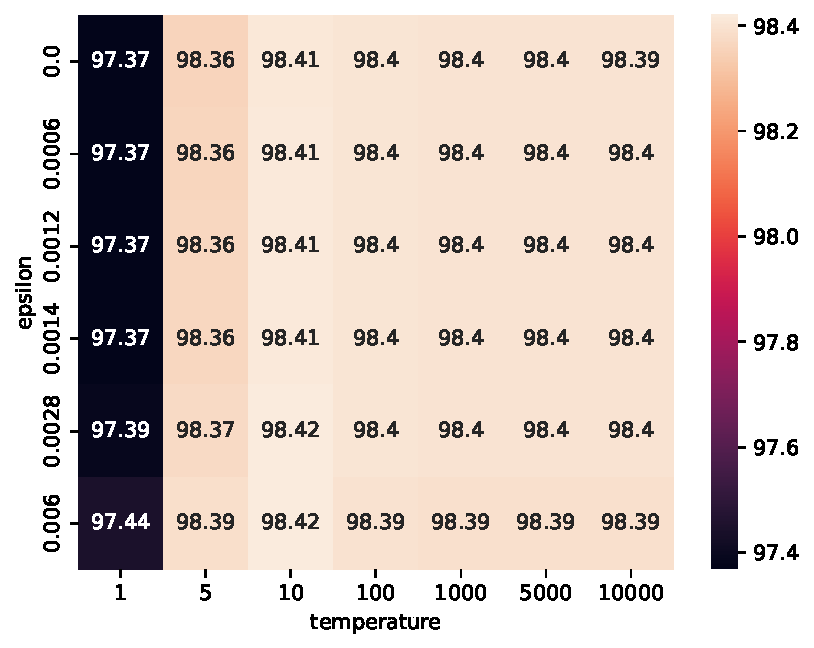
\includegraphics[width=\textwidth]{odin_grid_search.pdf}
        \caption{}
        \label{fig:odin_grid_search}
    \end{subfigure}%
    \caption{\textbf{(a) AUPR values for combined ODIN and MC Dropout techniques.} Analysis of the combined impact of ODIN techniques with MC Dropout (averaging over 100 stochastic forward passes), predictive entropy, and mutual information on AUPR values. The combination slightly reduces the performance of Entropy and Mutual Information by about $0.3\%$, with no significant impact on ODIN's performance.\\\textbf{(b) Grid search results of ODIN's AUPR values relative to hyperparameters $\epsilon$ and temperature.} Grid search results showing the influence of ODIN's hyperparameters $\epsilon$ and temperature on its AUPR values. The best result is achieved with a temperature of 10, yielding a $98.42\%$ AUPR, surpassing MCD with entropy. Temperature scaling alone enhances AUPR by $1\%$, while perturbation has a negligible impact, suggesting temperature scaling as the more effective parameter.}
\end{figure}

Considering ODIN's persistent underperformance, we hypothesized it might be due to suboptimal hyperparameters. The code we used suggested values for $ \epsilon $ of $0.006$ and $0.0006$, but also recommended trying $ \epsilon = 0.0014 $ at the same time. Moreover, the original paper sometimes employed high temperature values, up to $10000$. This led us to conduct a grid search, the results of which, showing AUPR values in relation to $ \epsilon $ and temperature, are depicted in \Cref{fig:odin_grid_search}.

The overall influence of these parameters can be noticeable, with a maximum variation of $1\%$ between the highest and lowest scores. Setting the temperature to $ 10 $ yielded the best result, achieving a $98.42\%$ AUPR, surpassing MCD with entropy which scored $98.25\%$. Setting the temperature to $ 1 $ essentially disables temperature scaling, allowing us to isolate the effect of perturbation, and vice versa for $ \epsilon = 0 $. Hence, the first cell serves as a baseline for comparison with other cells. The first line indicates that temperature scaling alone can enhance AUPR by $1\%$, a modest but significant improvement given the close scores. However, examining the first column reveals no discernible impact ($<0.08\%$) of perturbation at any $ \epsilon $ value, suggesting that combining both parameters achieves similar results to using temperature scaling alone. As the provided code uses a smaller epsilon for OOD data, we also replicated the grid search with this adjustment, which led to analogous findings.